\chapter{Methodology}

\section{Materials}

\begin{enumerate}
	\item Cylindrical neodymium magnet (Shown in \cref{fig:magnets}, Diameter: $\qty{1}{\centi\meter}$, Height: $\qty{1.5}{\centi\meter}$, Magnetic dipole moment: $\approx \qty{0.4}{\ampere^2\meter}$, Mass: $\qty{17.4}{\gram}$)
	\item Solenoid (Shown in \cref{fig:solenoid}, Diameter: $\qty{1.13}{\milli\meter}$, Height: $\qty{2.5}{\centi\meter}$, Winding amount: $74$, Wire radius: $\qty{1.50}{\milli\meter}$, Mass: $\qty{31.6}{\gram}$)
	\item $2$ pieces of cloth (One for absorbing the fall of the magnets, another for holding the solenoid in place)
	\item Oscilloscope
\end{enumerate}

\begin{figure}[ht]
	\centering
	\begin{subfigure}[c]{0.4\textwidth}
		\centering
		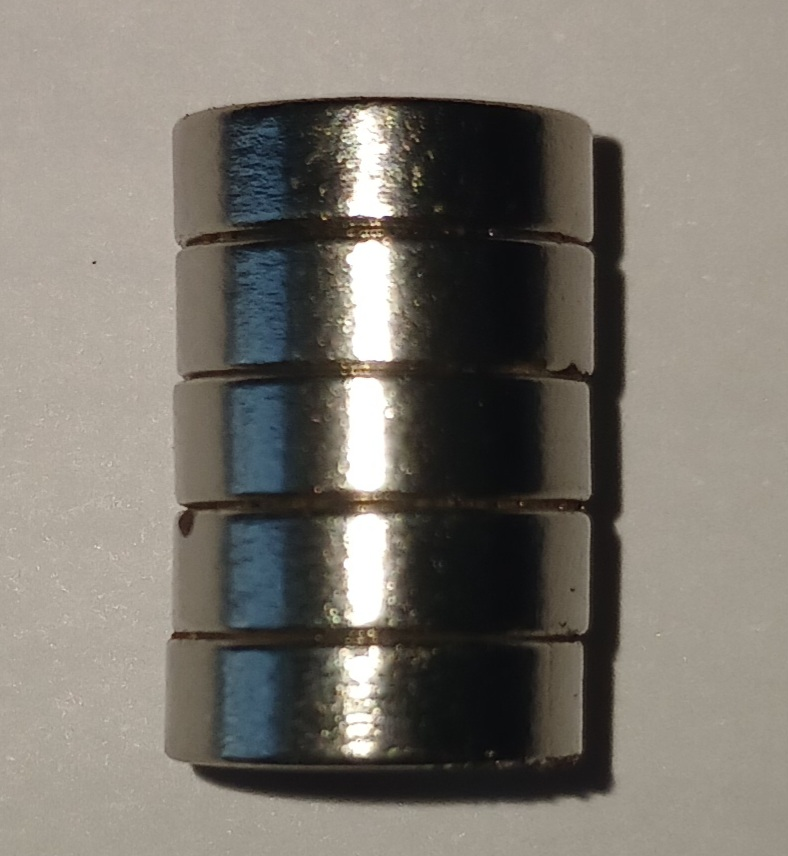
\includegraphics[height = 0.2\textheight]{figures/magnets.jpg}
		\caption{Cylindrical neodymium magnet}
		\label{fig:magnets}
	\end{subfigure}
	\begin{subfigure}[c]{0.4\textwidth}
		\centering
		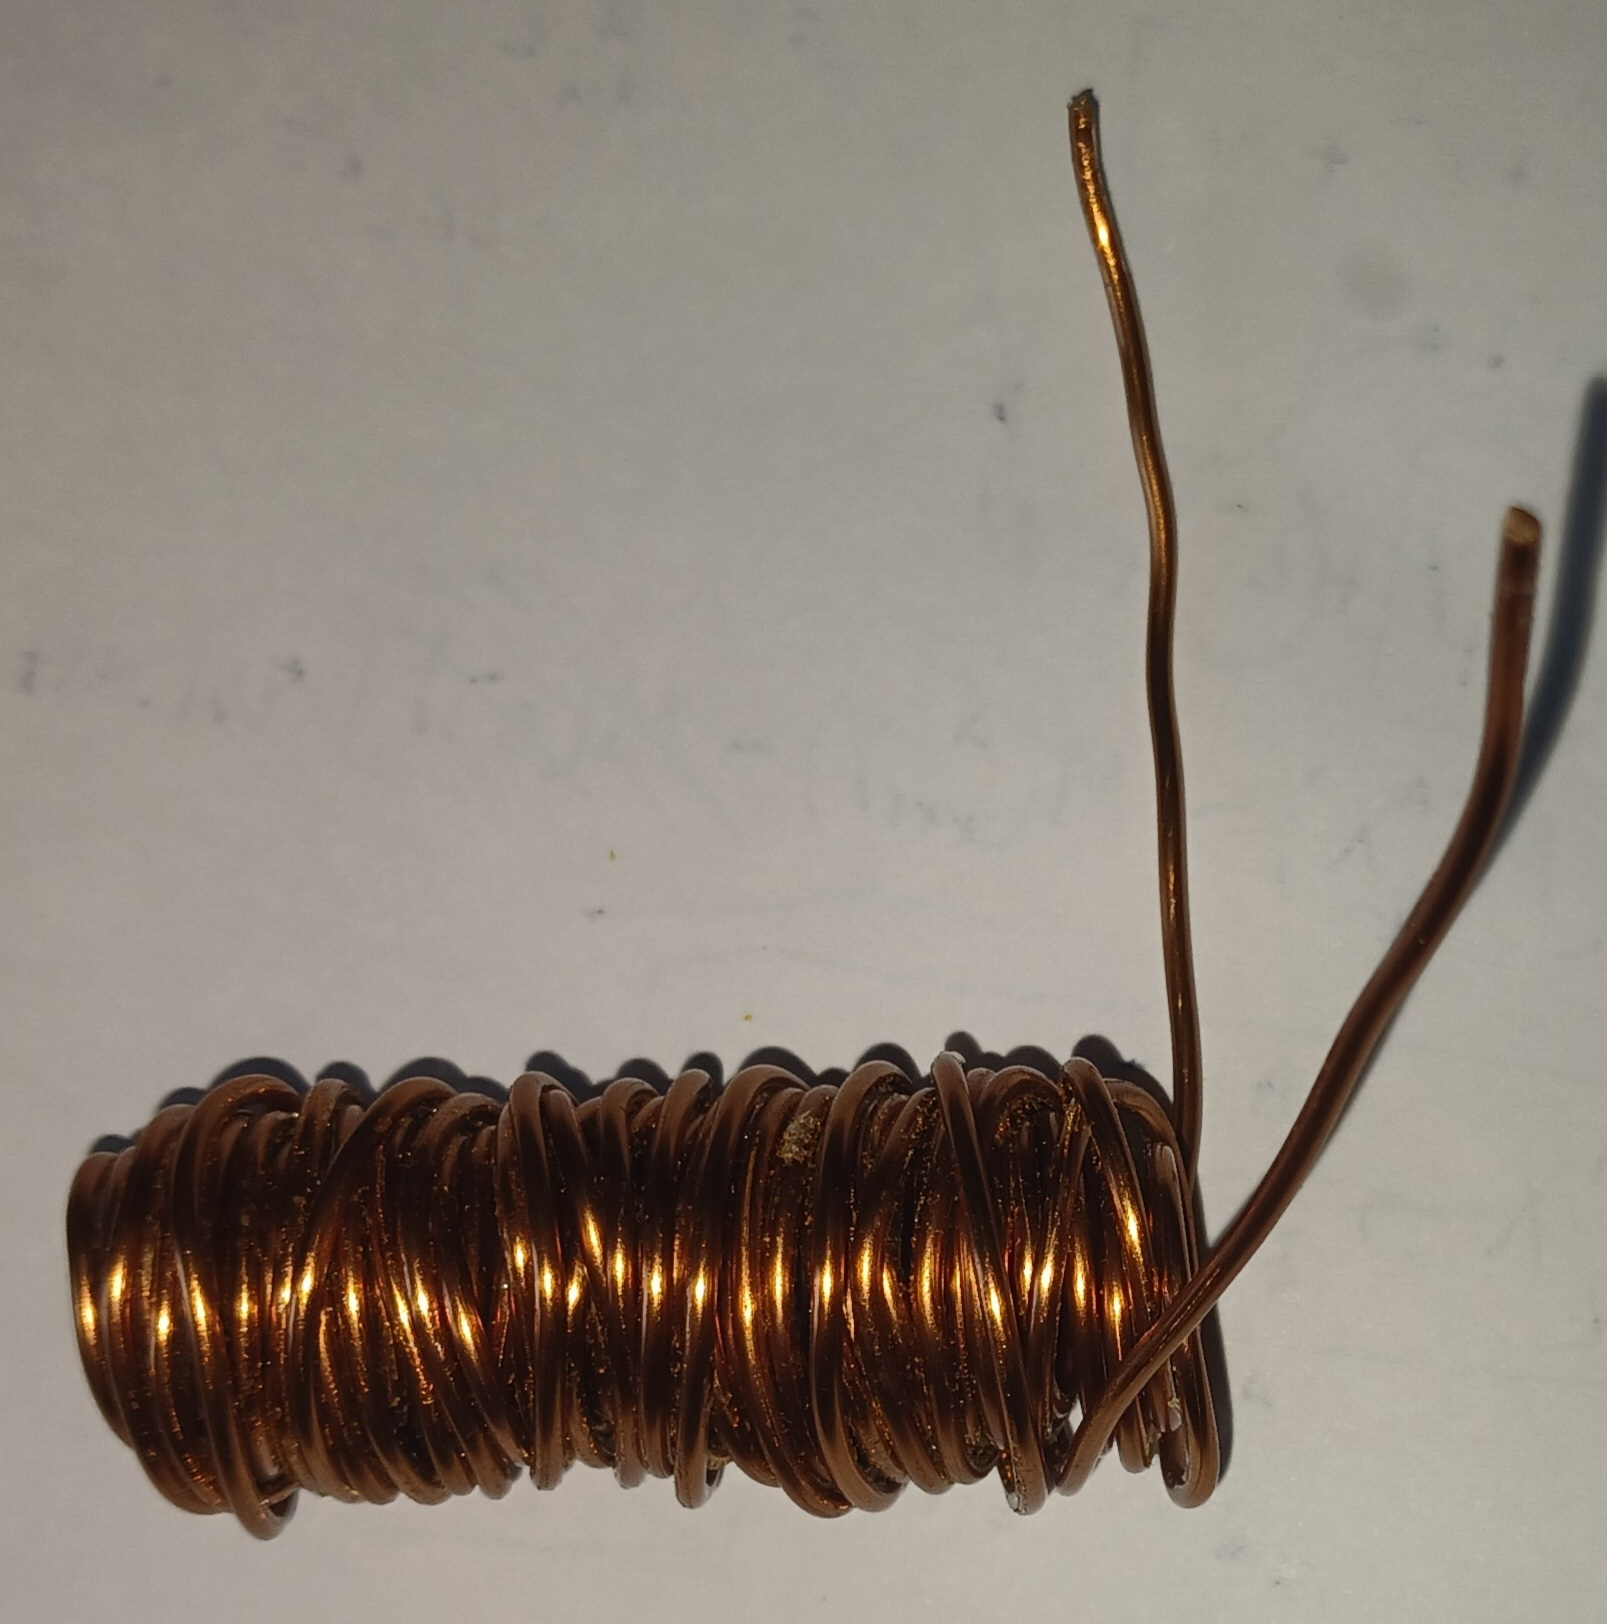
\includegraphics[height = 0.2\textheight]{figures/solenoid.jpg}
		\caption{Solenoid}
		\label{fig:solenoid}
	\end{subfigure}
	\caption{Materials used}
\end{figure}

\section{Methods}

\begin{enumerate}[noitemsep]
	\item Connect the solenoid to the oscilloscope.
	\item Place a piece of cloth below the solenoid.
	\item Hold the solenoid with the other piece of cloth $\qty{10}{\centi\meter}$ above the ground to prevent noise.
	\item Drop the magnets through the middle of the solenoid with varying heights from $\qty{0}{\centi\meter}$ to $\qty{14}{\centi\meter}$.
	\item Repeat five times for each height.
	\item Record the peak to peak voltage difference (Pk-Pk) from the oscilloscope.
\end{enumerate}

\section{Data analysis}
\label{sec:data-analysis}

The peak to peak voltage difference will be recorded onto a table, then plotted compared to the simulations.

To process the data and actually arrive at the gravitational acceleration, the Euler's method is used to simulate the dropping motion of the magnets with contributions from the Lenz law. Then, the position and velocity information is used to calculate the theoretical voltage. The code goes through every initial height in the range of $\qty{0}{\centi\meter}$ to $\qty{14}{\centi\meter}$ and gravitational acceleration values from $\qty{6}{\meter\per\second^2}$ to $\qty{12}{\meter\per\second^2}$. It then compares the theoretical result to the observed result and output the Earth's gravitational acceleration based on the minimum least mean squared error.

\begin{minted}{julia}
using Plots; plotlyjs()
using CUDA
using Statistics
using StatsBase
using Flux
# Variables declaration
global magneticPermeability = 1.256 * 10e-6
global solenoidLoopCount = 74
global solenoidRadius = 0.0058
global copperRadius = 0.00065
global solenoidLength = 2*π*solenoidRadius*solenoidLoopCount
global solenoidResistance = 1.68 * 10e-8 * solenoidLength
global copperDensity = 8850
global solenoidMass = solenoidLength * π * copperRadius^2 * copperDensity # 0.018
global magneticMoment = 0.4
global functionConst = (magneticMoment * magneticPermeability / 2)^2 * (12 * solenoidLoopCount * solenoidRadius) / (solenoidResistance * solenoidMass)
F(z) = functionConst * (2*z^3/(solenoidRadius^2 + z^2)^5 + z/(solenoidRadius^2 + z^2)^4)
# Voltage as a function of position of magnet and velocity
voltage(z, v) = @. - solenoidLoopCount * magneticPermeability * solenoidMass * z / 2 * v * (1/(solenoidRadius + z^2)^(3/2) - 3*z^2/(solenoidRadius^2 + z^2)^(5/2))

# Simulation configuration
global simTime = 0.4
global timeStep = 0.001
global timeInterval = CuArray(collect(0:timeStep:simTime))

# Simulating the voltage over time using Euler's method
function voltSim(initZ, gravitationalConst)
    posHistory = Float64.([initZ])
    veloHistory = Float64.([0.0])
    accel = - gravitationalConst
    for i in timeIndex #accel = - gravitationalConst + F(posHistory[i]) * veloHistory[i]
        nextVelo = veloHistory[i] + accel * timeStep
        push!(veloHistory, nextVelo)
        nextPos = posHistory[i] + veloHistory[i + 1] * timeStep
        push!(posHistory, nextPos)
    end
    minVoltage, maxVoltage = extrema(voltage.(posHistory, veloHistory))
    return abs(maxVoltage - minVoltage) # Return the predicted Pk-Pk output.
end

gVect = collect(9.52:0.00001:9.54)
zVect = collect(0:0.02:0.14)
gMat = gVect * ones(size(zVect, 1))'
zMat = ones(size(gMat, 1)) * zVect'

voltMat = voltSim.(zMat, gMat)
voltMatNorm = voltMat #.- minimum(voltMat, dims = 2)

data = [ # Raw data
    0.106  0.133  0.159  0.133  0.142;
    0.240  0.213  0.293  0.293  0.275;
    0.355  0.382  0.364  0.400  0.355;
    0.480  0.578  0.444  0.471  0.498;
    0.622  0.631  0.604  0.693  0.676;
    0.684  0.667  0.684  0.676  0.711;
    0.738  0.747  0.863  0.720  0.774;
    0.916  0.871  0.800  0.925  0.925;
] # Raw data, in millivolts
meanData = mean(data, dims = 2)

# Setup comparison
gVect = collect(6:0.00001:12)
zVect = collect(0:0.02:0.14)
gMat = gVect * ones(size(zVect, 1))'
zMat = ones(size(gMat, 1)) * zVect'
voltMat = voltSim.(zMat, gMat)

# Calculating errors
errorVect = []
rSqVect = []
# Error calculation
function rSquared(y, ypred)
    ss_res = sum((y .- ypred).^2)
    ss_tot = sum((y .- mean(y)).^2)
    return 1 - ss_res/ss_tot
end
for i in 1:size(gVect, 1)
    push!(errorVect, Flux.Losses.mse(normDat, voltMat'[:, i]))
    push!(rSqVect, rSquared(normDat, voltMat'[:, i]))
end
# Displaying the gravity
display(gVect[findall(x -> x == minimum(errorVect), errorVect)])
\end{minted}
